% The dynamic program of Section 5 visualized: Figure 1 of the paper (EJOR), unchanged.
% A set Z of jobs in three reference frames, with the profiles x at s_j and y at s_{j-1}.
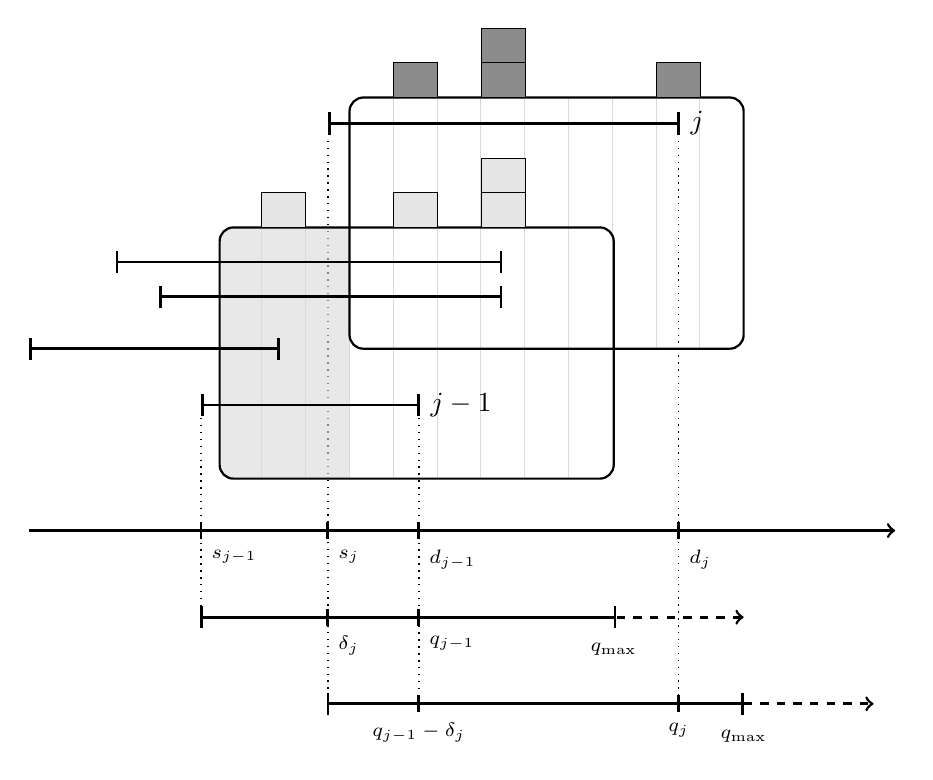
\begin{tikzpicture}[scale=1.1,yscale=1]

% Axis and ticks
\draw[line width=1, ->]
(0, -1) -- (10 , -1) node[] {};
\draw[line width=1, |-]
(3.5-1.526, -2) -- (3.5-1.5+4.75 , -2) node[] {};
\draw[line width=1,dashed, <-|]
 (3.5+4.75 , -2) -- (3.5-1.5+4.75, -2) node[] {};
 \draw[line width=1,dashed, ->]
 (3.5+4.75 , -3) -- (3.5+4.75+1.5, -3) node[] {};
\draw[line width=1, |-|]
(3.435, -3) -- (3.5+4.75, -3) node[below] {};
\node at (3.5+4.75, -3-0.375) {\scriptsize$q_{\max}$};
\node at (3.5-1.5+4.75, -2-0.375) {\scriptsize$q_{\max}$};

% }



\draw[line width=.5,dotted, -] (3.45, 3.5) -- (3.45, -3.1) node[below] {};
\draw[line width=1., -] (3.45, -.9) -- (3.45, -1.1) node[below right] {\scriptsize$s_{j}$};
\draw[line width=1., -] ((7.5, -.9) -- ((7.5, -1.1) node[below right] {\scriptsize$d_{j}$};
\draw[line width=1., -] ((6-1.5, -.9) -- ((6-1.5, -1.1) node[below right] {\scriptsize$d_{j-1}$};

\draw[line width=.5,dotted, -] (7.5, 3.5) -- (7.5, -3) node[below] {};
\draw[line width=1., -] (7.5, -2.9) -- (7.5, -3.1) node[below] {\scriptsize$q_{j}$};
% \draw[line width=1., -] (7.5, -1.9) -- (7.5, -2.1) node[below right] {\scriptsize$\delta_j+q_{j}$};


% Left gray half (manually shaded)
% Fill left half in gray
\fill[gray!30,opacity=.6]
  (2.0+0.2,-0.325) -- 
  (2.05+0.2,-0.35) -- 
  (2.1+0.2,-0.4) -- 
  (3.7,-0.4) -- 
  (3.7,2.5) -- 
  (2.1+0.2,2.5) -- 
  (2.0+0.2,2.4) -- 
  (2.0+0.2,2.5) -- 
  cycle;

% Histogram parameters
\def\xstart{3.5+0.2}
\def\xend{8.25}
\def\nbars{10}
\pgfmathsetmacro{\width}{(\xend - \xstart)/\nbars}



% Define rectangle corners
\def\xstart{2.2}
\def\xend{6.75}
\def\ystart{-0.4}
\def\yend{2.5}

% Number of vertical lines
\def\nlines{8}
% Draw vertical lines inside the rectangle
\pgfmathsetmacro{\spacing}{(\xend - \xstart)/(\nlines + 1)}
\foreach \i in {1,...,\nlines} {
    \pgfmathsetmacro{\x}{\xstart + \i * \spacing}
    \draw[thin,gray!30] (\x-0.017,\ystart) -- (\x-0.017,\yend);
}


% Define rectangle corners
\def\xstart{3.7}  % 3.5 + 0.2
\def\xend{8.25}
\def\ystart{1.1}
\def\yend{4.0}
% Number of vertical lines
\def\nlines{8}

\pgfmathsetmacro{\spacing}{(\xend - \xstart)/(\nlines + 1)}
\foreach \i in {1,...,\nlines} {
    \pgfmathsetmacro{\x}{\xstart + \i * \spacing}
    \draw[thin,gray!30] (\x,\ystart) -- (\x,\yend);
}

% Draw Rects
\draw[rounded corners=5pt, thick] (2.2,-0.4) rectangle (6.75,2.5);
\draw[rounded corners=5pt, thick] (3.5+0.2,1.1) rectangle (8.25,4.);


\draw[line width=.5,dotted, -] (1.985, .3) -- (1.985, -2.1) node[below] {};
\draw[line width=1., -] (1.985, -.9) -- (1.985, -1.1) node[below right] {\scriptsize$s_{j-1}$};


\draw[line width=.5,dotted, -] (6-1.5, .3) -- (6-1.5, -3) node[below] {};
\draw[line width=1., -] (6-1.5, -2.9) -- (6-1.5, -3.1) node[below] {\scriptsize$q_{j-1}-\delta_j$};
\draw[line width=1., -] (6-1.5, -1.9) -- (6-1.5, -2.1) node[below right] {\scriptsize$q_{j-1}$};


\draw[line width=1., -] (3.45, -1.9) -- (3.45, -2.1) node[below right] {\scriptsize$\delta_{j}$};



% jobs j and j-1
\draw[|-|,line width=1.,opacity=1.]
        (3.45 , 3.7) -- (7.5+.015, 3.7) node[right] {$j$};
\draw[|-|,line width=1.,opacity=1.]
        (1.985 , .45) -- (6-1.5+.015, .45) node[right] {$j-1$};

% The rest of the ints

        
\draw[|-|,line width=1.,opacity=1.]
        (3.6-1.5-.35-.25 , 1.7) -- (6-1.5+.015+0.95, 1.7) node[] {};
\draw[|-|,line width=1.,opacity=1.]
        (3.6-1.5-.35-.75 , 2.1) -- (6-1.5+.015+0.95, 2.1) node[] {};

\draw[|-|,
% gray!90,
line width=1.,opacity=1.]
        (.0 , 1.1) -- (2.9, 1.1) node[] {};



% The histogram

% q_j
\draw[fill=gray!90] (7.24,4.) rectangle ++(\width+.015,.4);

% middle
\draw[fill=gray!90] (7.24-4*\width-.04,4.4) rectangle ++(\width+.015,.4);
\draw[fill=gray!90] (7.24-4*\width-.04,4.) rectangle ++(\width+.015,.4);

% q_j-1
\draw[fill=gray!90] (7.24-6*\width-.0625,4.) rectangle ++(\width+.015,.4);

% previous
% \draw[fill=gray!30] (7.24-9*\width-.0625,4.) rectangle ++(\width+.015,.4);
\draw[fill=gray!20] (7.24-9*\width-.1,2.5) rectangle ++(\width+.015,.4);


% middle
\draw[fill=gray!20] (7.24-4*\width-.04,2.9) rectangle ++(\width+.015,.4);
\draw[fill=gray!20] (7.24-4*\width-.04,2.5) rectangle ++(\width+.015,.4);

% q_j-1
\draw[fill=gray!20] (7.24-6*\width-.0625,2.5) rectangle ++(\width+.015,.4);

\end{tikzpicture}
